\documentclass[11pt,a4paper]{article}

\usepackage[T1]{fontenc}
\usepackage[utf8]{inputenc}
\usepackage{mathptmx}
\usepackage{courier}
\usepackage[margin=2.5cm]{geometry}
\usepackage{amsmath}
\usepackage{booktabs}
\usepackage{graphicx}
\usepackage{xcolor}
\usepackage[numbers,sort&compress]{natbib}
\usepackage{xurl}
\usepackage[hidelinks]{hyperref}
\hypersetup{pdftitle={Reading the Format, Not the Facts: Artefacts in LLM-Optimised Evidence Inflate Multilingual Fact-Checking Scores},pdfauthor={Muzammal Hussain}}
\usepackage{caption}
\captionsetup{font=small,labelfont=bf}

\newcommand{\code}[1]{\texttt{#1}}
\setlength{\emergencystretch}{3em}

\title{\textbf{Reading the Format, Not the Facts:\\Artefacts in LLM-Optimised Evidence Inflate\\Multilingual Fact-Checking Scores}}
\author{Muzammal Hussain\\
\small Independent researcher, Glasgow, United Kingdom\\
\small \href{mailto:muzammal@masmatixinnovations.co.uk}{muzammal@masmatixinnovations.co.uk}\\
\small ORCID: \href{https://orcid.org/0009-0001-2570-5686}{0009-0001-2570-5686}}
\date{\small November 2026}

\begin{document}
\maketitle

\begin{abstract}
\noindent
RU22Fact pairs 16,033 claims about the Russia--Ukraine conflict in English, Ukrainian, Russian and Chinese with
evidence that a large language model retrieved from the web and summarised. On the official test split, character n-gram
models reach macro-F1 0.679 with claim and evidence, against 0.268 for the majority class; a classifier that sees no
words, only six format features, reaches 0.591, or 79\% of that gain. The marks differ by label: a search-engine
greeting in 95\% of Supported but 12\% of Refuted Russian evidence, and Ukrainian evidence of median length 107
characters for Supported but 2,830 for Refuted claims. Removing the marks and then deleting every verdict word
(\textit{false}, \textit{fake}, \ldots) leaves the scores unchanged: 0.989 on Ukrainian for character n-grams and
1.000 for fine-tuned XLM-R, whose overall score is 0.683. XLM-R and multilingual-E5 reach 0.997--1.000 on
Ukrainian and Russian with or without the marks. The label is carried by what kind of text the evidence is, a full
debunking article or a short news lead, so near-perfect scores measure recognising the genre, not verifying the
claim. We release code that rebuilds every number from the pinned data and propose format-only, artefact-removed
and verdict-masked baselines for evaluations on LLM-built evidence.
\end{abstract}

\section{Introduction}

Automated fact-checking is usually framed as deciding whether evidence supports or refutes a claim
\citep{thorne2018fever}. Evidence is expensive to collect, and recent datasets use large language models to search the
web and condense what they find. RU22Fact \citep{zeng2024ru22fact} does this for 16,033 fact-checked claims about the
Russia--Ukraine conflict in four languages, and reports that such optimised evidence improves verification.

A dataset of this kind can teach a shortcut. Work on natural language inference showed that hypothesis-only models
beat the majority baseline on many datasets \citep{poliak2018hypothesis,gururangan2018annotation}, and on FEVER
claim-only classifiers performed competitively with evidence-aware models \citep{schuster2019debiasing}. When the
evidence itself is produced by a tool, the tool's habits can leave marks that differ by label. If evidence for true
claims is formatted differently from evidence for false ones, a model can read the format instead of the content.

We measure this on RU22Fact. Our questions are: (1) How much of the label can be predicted from the evidence's format
alone? (2) Does removing the format marks reduce the score of a model that reads the evidence? (3) Do models rely on the
verdict words in the evidence? (4) How do these effects differ across the four languages? The models are deliberately simple
and transparent, because the point is to audit the data, not to propose a verifier.

\section{Related work}

Hypothesis-only and claim-only baselines are the standard tool for finding label cues in one input
\citep{poliak2018hypothesis,gururangan2018annotation,schuster2019debiasing}. Our format-only probe applies the same
idea to the evidence, with features that carry no words at all. AVeriTeC \citep{schlichtkrull2023averitec} shows the
other side of the problem: it collects evidence through question answering on the open web and removes evidence
published after the claim, to avoid temporal leakage, whereas RU22Fact's evidence was retrieved and summarised by a
model after the fact-checks existed. X-FACT \citep{gupta2021xfact} introduced multilingual
fact-checking with zero-shot transfer across languages; we report transfer from English for comparison. Selective
classification \citep{geifman2017selective} lets a model abstain on its least confident inputs; we report
risk-coverage results because a verifier for conflict claims should be able to say it does not know.

\section{Data and method}

\paragraph{Data.} RU22Fact \citep{zeng2024ru22fact} provides train, validation and test splits with the labels
Supported, Refuted and NEI (not enough information), the claim, the LLM-optimised evidence and a reference explanation.
We use the files at commit \code{c467abb} of the authors' repository and check their SHA-256 digests. Two rows
(one in train and one in test) have shifted columns and no language and are dropped, leaving 16,031 claims. The test
split has 1,741 English, 704 Ukrainian, 465 Russian and 305 Chinese claims; Ukrainian and Russian have no NEI claims.
The reference explanation states the verdict and is never used as input.

\paragraph{Models.} For each input (claim, evidence, claim and evidence) we fit a character 2--5-gram TF-IDF model with
class-balanced logistic regression, choose $C \in \{0.3, 1, 3\}$ on validation macro-F1 and score the test split once.
Character n-grams work for all four scripts without language-specific tools.

\paragraph{Neural encoders.} To test whether the findings hold beyond lexical models, we fine-tune two multilingual
encoders on claim--evidence pairs: XLM-R base \citep{conneau2020xlmr} and multilingual-E5 base
\citep{wang2024me5}, a retrieval-tuned encoder of the same size. Inputs are claim--evidence pairs of at most 256 tokens, with the evidence truncated; training uses AdamW with learning rate $2\times10^{-5}$, batch size 32, 3 epochs, class-weighted cross-entropy
and mixed precision on one T4 GPU. The epoch with the best validation macro-F1 is scored on test. Each model is
trained with three seeds on raw evidence and on artefact-removed evidence, and we report mean and standard deviation.

\paragraph{Format-only probe.} A logistic regression on six features of the evidence that contain no words: whether it
mentions the search engine (Bing, whose greeting appears in many evidence texts), whether it starts with a
\code{[1]} citation marker or with list numbering, its log length, and its shares of Latin letters and digits, with
language indicators and their interactions with the first four features.

\paragraph{Artefact removal.} We delete sentences that mention the search engine, citation markers such as
\code{[1]:}, list numbering and markdown emphasis, and refit the evidence model and the probe with $C=1$ (the value
selected for raw evidence). A second variant also keeps only the first 300 characters, to remove most of the length
difference.

\paragraph{Verdict words.} For each language, a short list of words with which fact-checkers state a verdict
(for example \textit{false}, \textit{misleading} and \textit{no evidence} in English, \textit{fake},
\textit{untrue} and \textit{refuted} in Ukrainian and Russian), and the share of evidence texts containing one.
To test whether models rely on these words, we also delete every word that contains one (in Chinese, the cue itself)
from the artefact-removed evidence and refit the lexical models and XLM-R on this verdict-masked evidence.

\paragraph{Metrics.} Macro-F1 over the three labels is the main metric because NEI is rare; per language it is taken
over the labels present. Test intervals are 95\% percentile bootstrap intervals over claims (1,000 resamples). For
abstention we rank claims by the top predicted probability and report accuracy on the most confident 50\% and 80\%
and the area under the risk-coverage curve (AURC; lower is better).

\section{Results}

\begin{table}[t]
\centering\small
\caption{Test macro-F1 overall (95\% bootstrap interval) and per language. Per-language scores for Ukrainian and
Russian are over Supported and Refuted only.}
\label{tab:main}
\setlength{\tabcolsep}{4pt}
\begin{tabular}{lccccc}
\toprule
Input & Overall & en & uk & ru & zh \\
\midrule
Majority class (Supported) & 0.268 & & & & \\
Claim & 0.614 [0.594, 0.633] & 0.584 & 0.868 & 0.950 & 0.572 \\
Evidence & 0.677 [0.655, 0.696] & 0.631 & 0.989 & 0.995 & 0.696 \\
Claim and evidence & 0.679 [0.659, 0.698] & 0.631 & 0.989 & 0.995 & 0.713 \\
\midrule
Evidence format only (no words) & 0.591 [0.574, 0.609] & 0.543 & 0.944 & 0.931 & 0.352 \\
\quad after artefact removal & 0.396 & 0.117 & 0.944 & 0.493 & 0.330 \\
\quad after removal, first 300 characters & 0.357 & 0.046 & 0.939 & 0.463 & 0.096 \\
\midrule
Evidence after artefact removal & 0.678 [0.657, 0.696] & 0.630 & 0.989 & 0.971 & 0.710 \\
\quad first 300 characters & 0.636 [0.618, 0.655] & 0.581 & 0.970 & 0.931 & 0.685 \\
\midrule
Claim and evidence, trained on English only & & 0.641 & 0.236 & 0.927 & 0.503 \\
\bottomrule
\end{tabular}
\end{table}

\paragraph{The format predicts the label.} The claim-and-evidence model reaches 0.679 macro-F1 and 85.9\% accuracy
(Table~\ref{tab:main}). The format-only probe, which reads no words, reaches 0.591 and 76.1\%: 79\% of the gain of the
full model over the majority class. The marks differ sharply by label. In Russian, 94.8\% of Supported but 11.7\% of
Refuted evidence mentions the search engine. In English, 83.2\% of Supported and 12.7\% of Refuted evidence starts
with \code{[1]}. In Ukrainian, the median evidence is 107 characters for Supported and 2,830 for Refuted claims.
Figure~\ref{fig:lang} shows the result per language.

\begin{figure}[t]
  \centering
  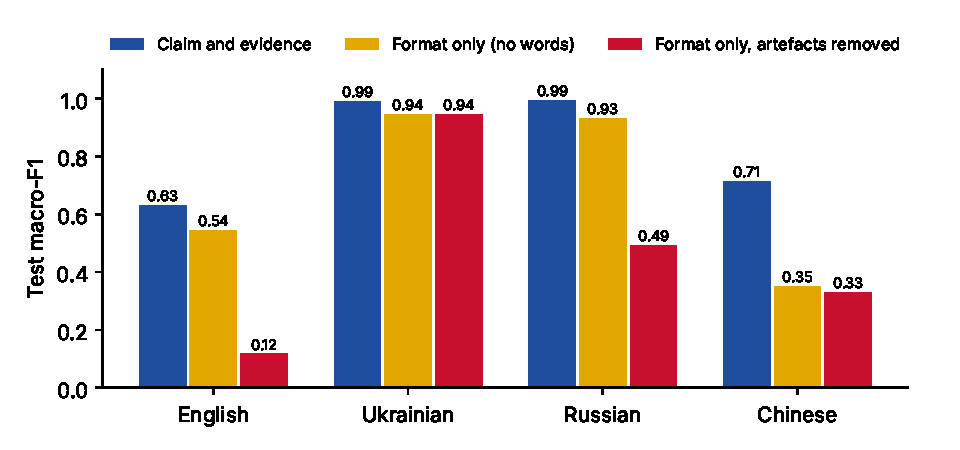
\includegraphics[width=0.85\linewidth]{figures/fig_format_probe.pdf}
  \caption{Test macro-F1 per language for the claim-and-evidence model, the format-only probe, and the probe after
  artefact removal. Ukrainian and Russian are scored over Supported and Refuted.}
  \label{fig:lang}
\end{figure}

\paragraph{Removing the marks removes the format signal, not the score.} After artefact removal the probe falls to
0.396 overall, to 0.117 in English and to 0.493 in Russian. The evidence model, however, keeps 0.678, and 0.636 with
only the first 300 characters. It therefore also learns from the content. In Ukrainian the probe stays at 0.944 even
after truncation, because the short Supported texts are still shorter than 300 characters.

\paragraph{Verdict words are present but are not what the models use.} In Ukrainian, 77.5\% of Refuted evidence
contains a debunking word, against 0.6\% of Supported evidence; the gap is smaller elsewhere (29.8\% against 5.9\% in
Russian, 28.6\% against 5.2\% in English, 9.4\% against 3.7\% in Chinese). Deleting these words, however, changes
nothing: on artefact-removed and verdict-masked evidence the character n-gram evidence model scores 0.684 overall
(0.678 before masking), 0.989 on Ukrainian and 0.976 on Russian, and fine-tuned XLM-R scores 0.683 overall and
1.000 and 0.993 on Ukrainian and Russian (Table~\ref{tab:neural}). What remains is the kind of text: Refuted
Ukrainian evidence reads like the fact-check article itself, Supported evidence like a short news lead, and their
lengths differ twentyfold. Near-perfect scores in Ukrainian and Russian therefore come from recognising the genre and
format of the evidence, not from comparing the claim with independent evidence.

\begin{table}[t]
\centering\small
\caption{Fine-tuned encoders on claim and evidence: test macro-F1, mean $\pm$ SD over three seeds, and per language
(mean). Artefact removal as in Table~\ref{tab:main}; verdict words deleted as in Section~3.}
\label{tab:neural}
\setlength{\tabcolsep}{4pt}
\begin{tabular}{llccccc}
\toprule
Model & Evidence & Overall & en & uk & ru & zh \\
\midrule
XLM-R base & raw & 0.689 $\pm$ 0.003 & 0.643 & 1.000 & 0.997 & 0.676 \\
 & artefacts removed & 0.691 $\pm$ 0.005 & 0.644 & 0.999 & 0.997 & 0.700 \\
 & \quad and verdict words deleted & 0.683 $\pm$ 0.004 & 0.633 & 1.000 & 0.993 & 0.669 \\
multilingual-E5 base & raw & 0.701 $\pm$ 0.008 & 0.652 & 0.999 & 0.999 & 0.709 \\
 & artefacts removed & 0.697 $\pm$ 0.008 & 0.647 & 0.999 & 0.997 & 0.710 \\
\bottomrule
\end{tabular}
\end{table}

\paragraph{Neural encoders show the same picture.} Fine-tuned XLM-R and multilingual-E5 reach 0.689 and 0.701,
only one to two points above the character n-gram model (Table~\ref{tab:neural}). Artefact removal changes neither
score by more than the seed spread, and both encoders stay at 0.997--1.000 on Ukrainian and Russian. Larger models
therefore do not reduce the dependence on what kind of text the evidence is; they recognise it at least as well.
English and Chinese, where Supported and Refuted evidence look more alike, stay at 0.63--0.71 for every model.

\paragraph{Claims carry cues too.} The claim alone reaches 0.614, far above the majority class, as on FEVER
\citep{schuster2019debiasing}. In Russian the claim alone reaches 0.950.

\paragraph{NEI and abstention.} NEI is the hard class: F1 0.262 with claim and evidence, against 0.938 for Supported
and 0.836 for Refuted. Answering only the most confident half of the test claims raises accuracy from 85.9\% to
98.1\% (80\%: 93.2\%; AURC 0.034). Abstention works well here partly because the artefacts make many decisions easy.

\paragraph{Transfer.} Trained on English only, the model scores 0.236 on Ukrainian and 0.503 on Chinese, but 0.927 on
Russian. Character n-grams learned from English cannot read Russian; the Russian score comes from shared marks such as
the search-engine greeting.

\section{Discussion}

RU22Fact is a valuable resource: it is multilingual, it covers a conflict where misinformation matters, and it was
built transparently. Its evidence, however, was not written independently of the label. The search tool's greeting
and citation style differ between claims later labelled true and false, and for Ukrainian the evidence for false claims
is often the debunking text. A verifier evaluated on it can score highly without verifying anything. This does not
make the dataset unusable; it means that results on it need controls. We suggest three: report a format-only
baseline, report scores after removing tool artefacts, and check whether scores survive deleting the verdict words.
All three are cheap; the lexical versions run on a laptop.

For conflict-related claims in particular, a system that appears accurate because it recognises a debunking article
would fail exactly where it is needed: on new claims for which no fact-check exists yet.

\section{Limitations}

Besides the lexical models we test two base-size encoders; larger models and LLM agents that retrieve their own
evidence may use the cues to a different degree, which we have not measured. The artefact removal targets the marks we found and cannot remove all format or
verdict signal. The verdict-word lists are short and hand-made; masking them removes the listed words but not every way of stating
a verdict, so it bounds rather than removes the verdict signal. We did not equalise evidence length or genre, which
is what remains. We rely on the released labels and do not re-verify any claim. Ukrainian and Russian have no NEI claims, so
their scores are not comparable with English and Chinese. Lexical results come from one fit; their bootstrap intervals cover sampling of test claims, not training
variation. The encoder results use three seeds, which bounds training variation but gives no test-sampling interval.

\section{Conclusion}

On RU22Fact, a classifier that reads no words of the evidence reaches 79\% of the gain of a classifier that reads
claim and evidence. Removing the format marks and deleting the verdict words leaves the scores unchanged: in
Ukrainian and Russian the label is carried by whether the evidence is a debunking article or a news lead, and
fine-tuned multilingual encoders recognise this as well as character n-grams. Evaluations of fact-checkers on LLM-built evidence should report format-only and artefact-removed
baselines alongside their main scores.

\section*{Code and data availability}

Code, tests and the archived results are at \url{https://github.com/MHKhan50/multilingual-factcheck-artefacts} (software:
\href{https://doi.org/10.5281/zenodo.24370943}{doi:10.5281/zenodo.24370943}). The data are not redistributed:
\code{civintel ru22fact-download} fetches them from the authors' repository at a pinned commit and checks their
SHA-256 digests, and \code{civintel ru22fact-verify} reproduces every number in this paper in about 15 minutes on a
laptop CPU. \code{civintel ru22fact-neural} and the notebooks \code{notebooks/kaggle\_xlmr.ipynb} and
\code{notebooks/kaggle\_me5.ipynb} reproduce the encoder results on a free Kaggle T4 GPU (about 1 hour per model).

\bibliographystyle{plainnat}
\bibliography{references}

\end{document}
